% ------------------------------------------------------------------------------
% TYPO3 CMS 8.0 - What's New (French Version)
%
% @author	Patrick Lobacher <patrick@lobacher.de> and Michael Schams <schams.net>
% @license	Creative Commons BY-NC-SA 3.0
% @link		http://typo3.org/download/release-notes/whats-new/
% @language	French
% ------------------------------------------------------------------------------
% LTXE-CHAPTER-UID:		d71b4b88-f79b2343-d2b356bf-452cef81
% LTXE-CHAPTER-NAME:	Backend User Interface
% ------------------------------------------------------------------------------

\section{Interface Utilisateur Backend}
\begin{frame}[fragile]
	\frametitle{Interface Utilisateur Backend}

	\begin{center}\huge{Chapitre 1~:}\end{center}
	\begin{center}\huge{\color{typo3darkgrey}\textbf{Interface Utilisateur Backend}}\end{center}

\end{frame}

% ------------------------------------------------------------------------------
% LTXE-SLIDE-START
% LTXE-SLIDE-UID:		4b14ff37-4c8988a5-5a1ee4eb-0b3880e3
% LTXE-SLIDE-ORIGIN:	d8599a04-11b4fa8c-9be5812a-715820e1 English
% LTXE-SLIDE-ORIGIN:	ef1d6d8c-0db67396-dedb5814-1767169f German
% LTXE-SLIDE-TITLE:		Recover pages recursively to top of rootline
% LTXE-SLIDE-REFERENCE:	!Feature-1835-RecoverPagesRecursivelyToTop.rst
% ------------------------------------------------------------------------------
\begin{frame}[fragile]
	\frametitle{Interface Utilisateur Backend}
	\framesubtitle{Restaurer les pages récursivement à la racine}

	La Corbeille supporte la restauration récursive des pages supprimées à la racine.
	Cette fonctionnalité n'est disponible que pour les administrateurs en raison des permissions requises.

	\begin{figure}
		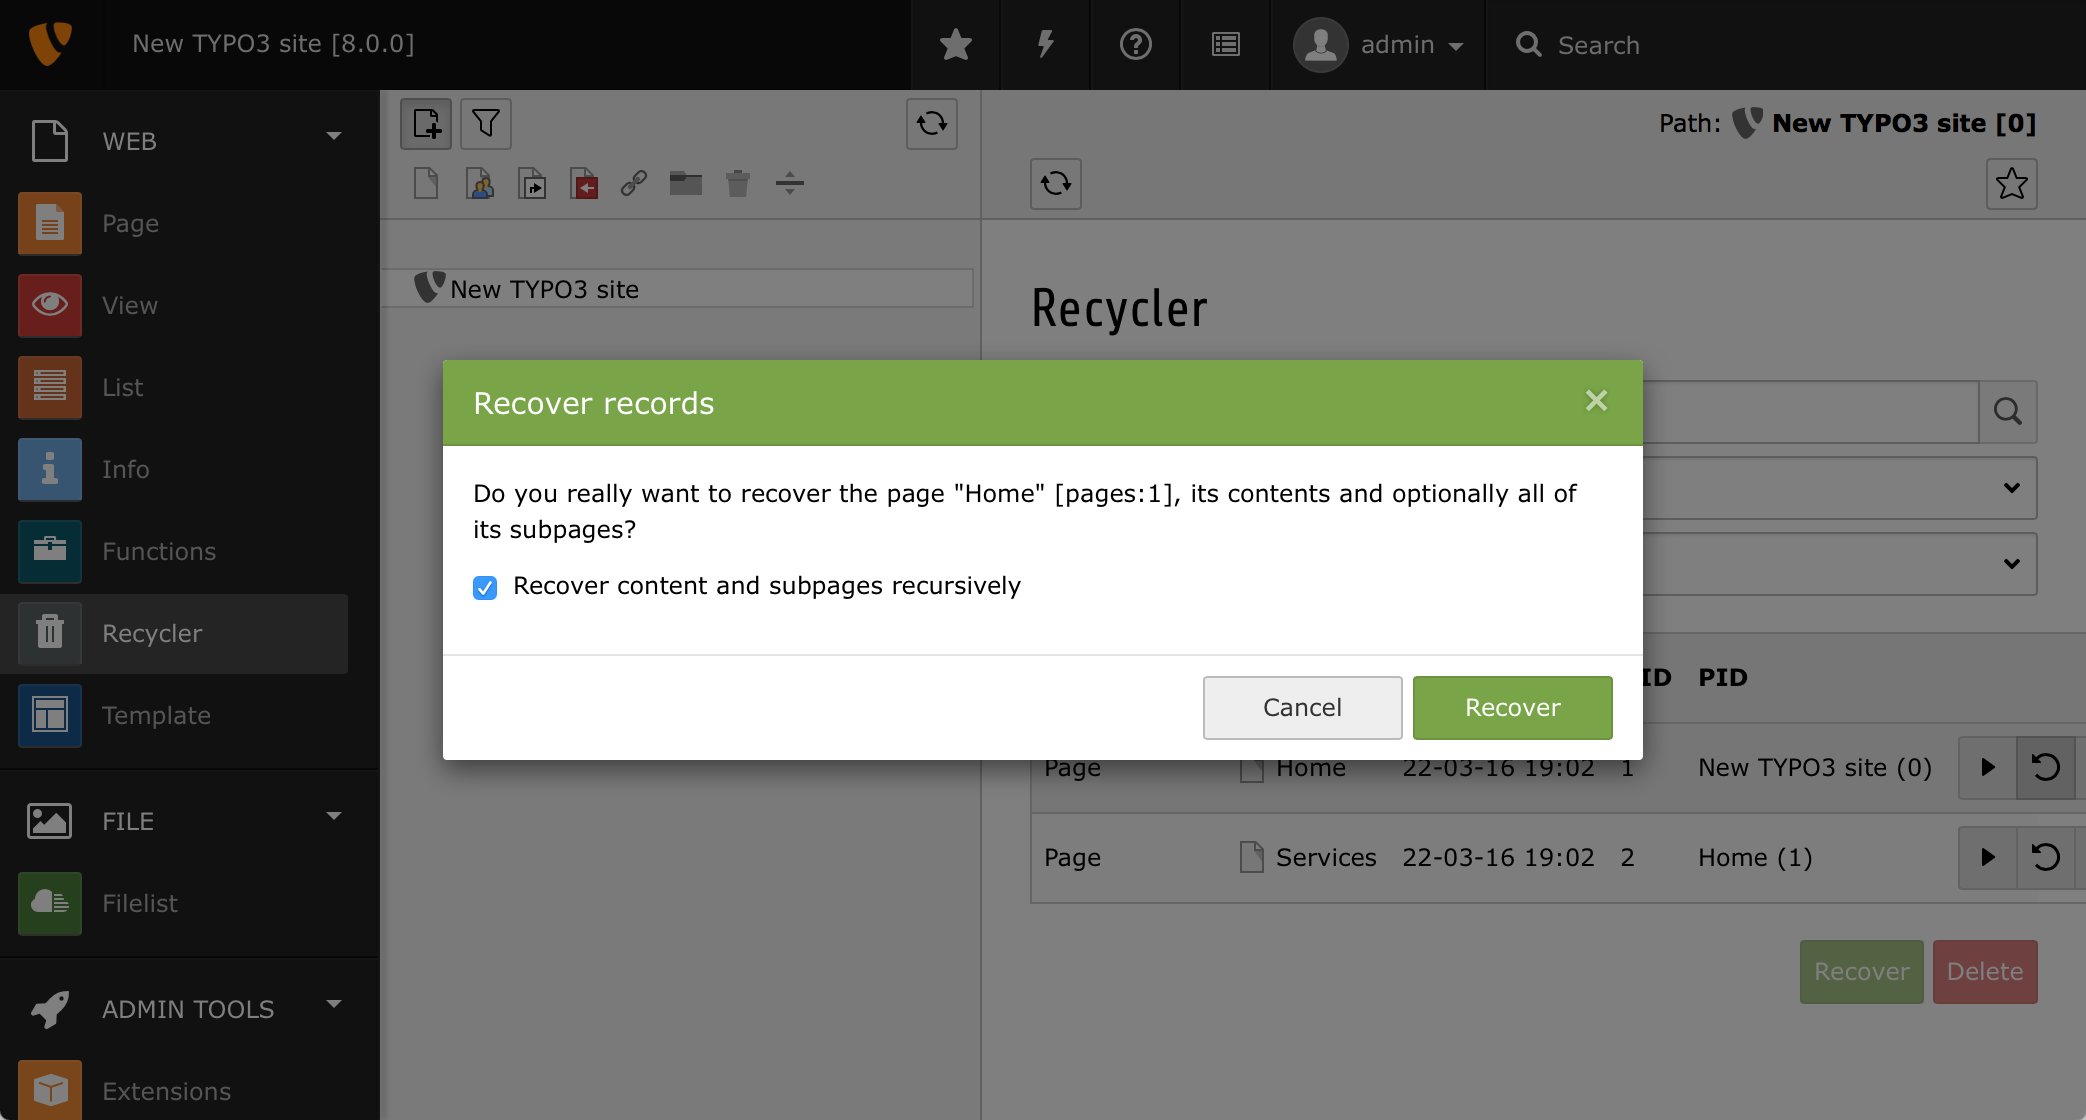
\includegraphics[width=0.70\linewidth]{BackendUserInterface/1835.png}
	\end{figure}

\end{frame}

% ------------------------------------------------------------------------------
% LTXE-SLIDE-START
% LTXE-SLIDE-UID:		eaa18646-526cd7b8-60306bfa-9083995c
% LTXE-SLIDE-ORIGIN:	04855567-dac16e24-f5274c64-f1d49c36 English
% LTXE-SLIDE-TITLE:		EXT:form - Directly load form wizard as inline wizard
% LTXE-SLIDE-REFERENCE:	!Feature-69394-EXTform-DirectlyLoadFormWizardAsInlineWizard.rst
% ------------------------------------------------------------------------------
\begin{frame}[fragile]
	\frametitle{Interface Utilisateur Backend}
	\framesubtitle{Chargement sur place de l'assistant formulaire}

	L'assistant de EXT:form est chargé directement en tant qu'assistant sur place.
	Il n'y a plus besoin d'enregistrer et recharger le nouvel élément de contenu
	afin d'ouvrir l'assistant. C'est une importante amélioration de l'usabilité.

	\begin{figure}
		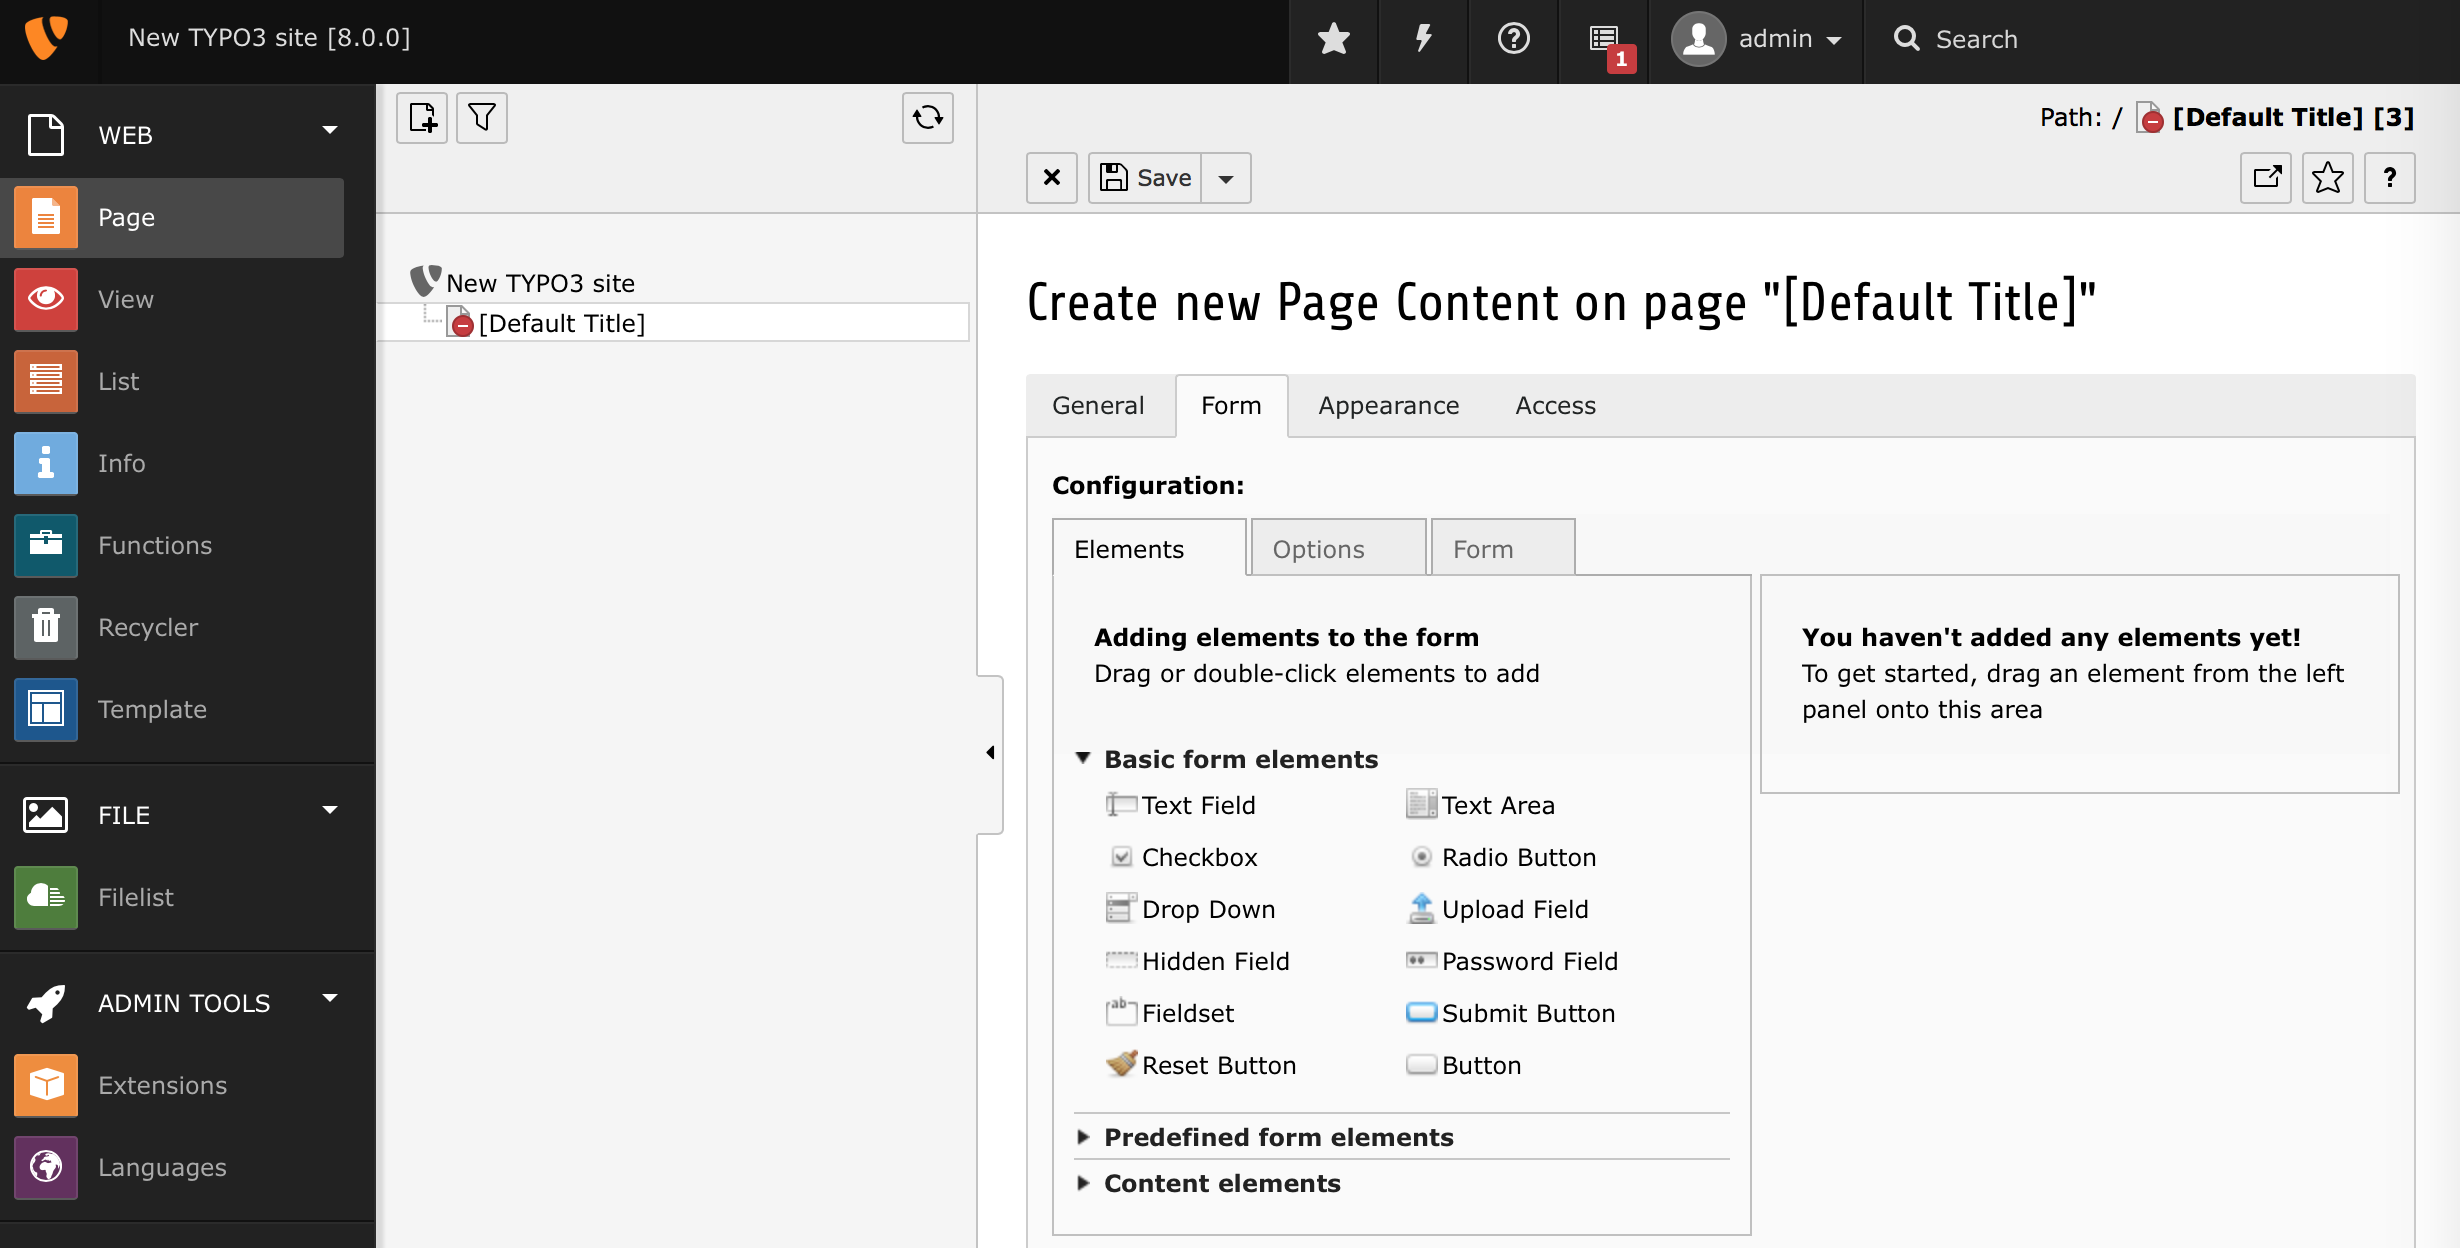
\includegraphics[width=0.70\linewidth]{BackendUserInterface/69394.png}
	\end{figure}

\end{frame}

% ------------------------------------------------------------------------------
% LTXE-SLIDE-START
% LTXE-SLIDE-UID:		f91b4717-7ae80430-0a833eb0-f3677545
% LTXE-SLIDE-ORIGIN:	fd6d762a-b268caf0-cb6f9195-f553e035 English
% LTXE-SLIDE-TITLE:		Set the alternative backend logo via Extension Manager
% LTXE-SLIDE-REFERENCE:	!Feature-74109-SetTheAlternativeBackendLogoViaExtensionManager.rst
% ------------------------------------------------------------------------------
\begin{frame}[fragile]
	\frametitle{Interface Utilisateur Backend}
	\framesubtitle{Définir un logo Backend alternatif via le gestionnaire d'extensions}

	Le logo du Backend dans le coin haut gauche est configurable dans la configuration
	de l'extension backend dans le gestionnaire d'extensions.\newline
	Les options de configuration sont~:

	\begin{itemize}
		\item chemin relatif à l'instance de TYPO3 vers une ressource\newline
			\smaller
				ex. "\texttt{fileadmin/images/my-background.jpg}"
			\normalsize

		\item chemin vers une ressource d'extension\newline
			\smaller
				ex. "\texttt{EXT:my\_theme/Resources/Public/Images/my-background.jpg}"
			\normalsize

		\item adresse d'une ressource externe\newline
			\smaller
				ex. "\texttt{//example.com/my-background.png}"
			\normalsize

	\end{itemize}

	\begin{figure}
		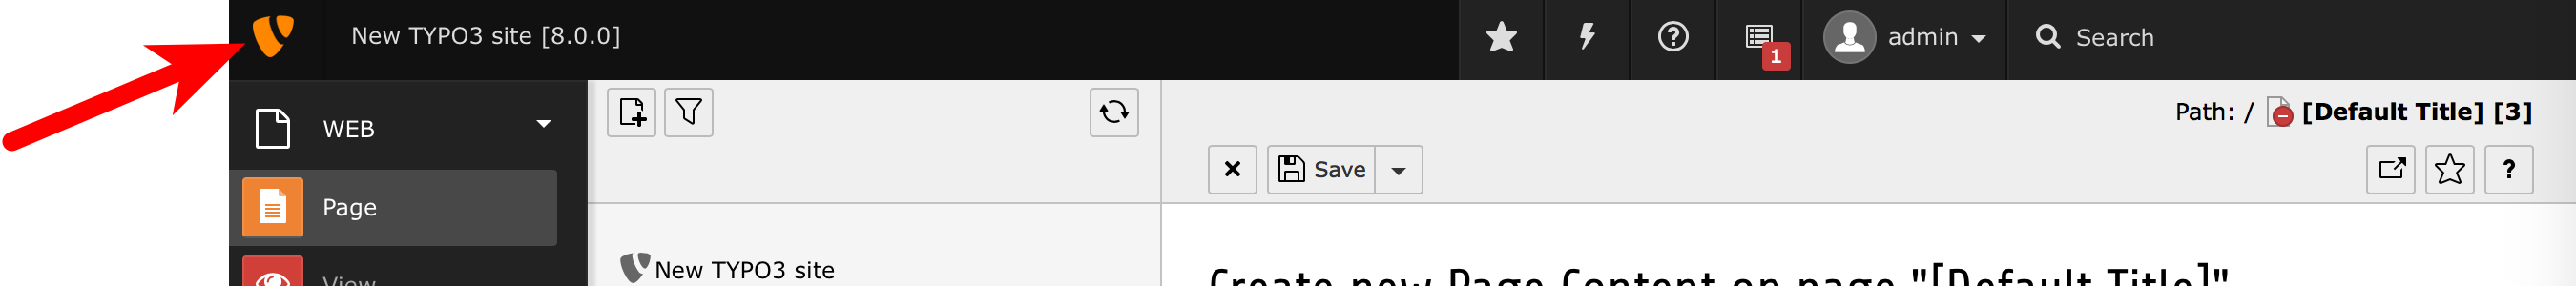
\includegraphics[width=0.7\linewidth]{BackendUserInterface/74109.png}
	\end{figure}

\end{frame}

% ------------------------------------------------------------------------------
% LTXE-SLIDE-START
% LTXE-SLIDE-UID:		a18edcbf-90159673-f3c1abdd-df0a5627
% LTXE-SLIDE-ORIGIN:	ab5ef36b-c670fbea-fd6d762a-cb6f9195 English
% LTXE-SLIDE-TITLE:		Page module: drag and drop supports copying now
% LTXE-SLIDE-REFERENCE:	!Feature-74179-PageModuleDragDropCanDoCopiesViaCTRLKeyNow.rst
% ------------------------------------------------------------------------------
\begin{frame}[fragile]
	\frametitle{Interface Utilisateur Backend}
	\framesubtitle{Pages~: copie d'élément en glisser-déposer}

	En plus de la fonctionnalité habituelle de glisser-déposer dans le module page (qui \textit{déplace} les
	éléments de contenu), des copies peuvent être créées~: maintenir la touche CTRL lors du dépôt pour créer
	une copie de l'élément attrapé. À la fin de l'opération, le module page se recharge pour créer le nouvel
	élément avec toutes les informations nécessaires.

	\begin{figure}
		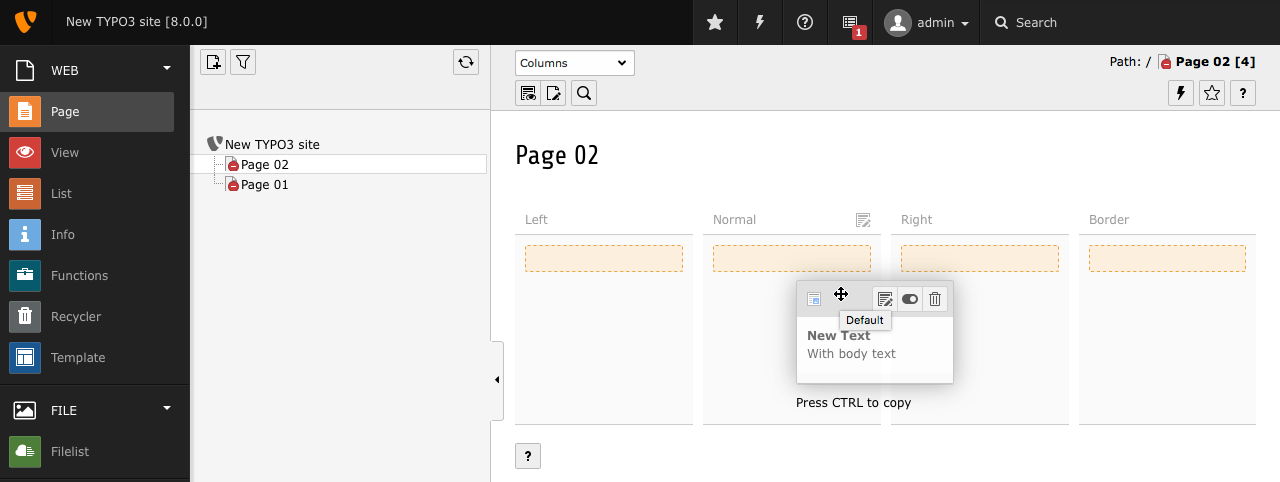
\includegraphics[width=0.7\linewidth]{BackendUserInterface/74179.png}
	\end{figure}

\end{frame}

% ------------------------------------------------------------------------------
